
\section{Geometría afín}

\subsection{Vectores y sistemas de referencia}





\subsection{Ecuaciones de la recta y del plano}

\obs Dado que la única manera que tenemos de determinar los puntos es a través de vectores de posición, utilizaremos $\vec{p} = (x,y,z)$ de forma equivalente a $[\vec{OP}]$ para referirnos a un punto cualquiera del espacio, al que accedemos a través de su vector de posición.

Formas de determinar una recta:
\begin{enumerate}
  \item Un punto (o su vector de posición) y un vector director.
  \subitem Dos puntos (se reduce al caso anterior)
  \subitem Un punto y una condición de paralelismo (se reduce al primer caso)
  \item Dos planos secantes.
  \item Un punto y un plano perpendicular (se verá en geometría euclídea).
\end{enumerate}

\obs Como todo con lo que vamos a trabajar son operaciones con vectores con coordenadas en un sistema de referencia, en realidad el punto de origen del sistema de referencia no es relevante. 
%
%(Ver ejemplo \ref{example::origen_ref}).

\subsubsection{Ecuaciones de la recta}

La 
%
\concept[Ecuación de la recta\IS vectorial]{ecuación vectorial de la recta} 
%
$r$ determinada por el punto $A\in\mathcal{E}_3$, cuyo vector de posición es $\vec{a}\in\mathcal{V}^3$, con vector director $\vec{u_r}\in\mathcal{V}^3 $  es 

\[ r: \vec{p} = \vec{a} + \lambda \vec{u_r}\]

donde $\lambda\in\real, \forall P\in\mathcal{E}_3$ (ver \fref{fig::recta_ecuacion_vectorial})
%
De esta manera quedan determinados los vectores de posición de todos los puntos de la recta $r$.


\begin{figure}[hptb]
    \centering
    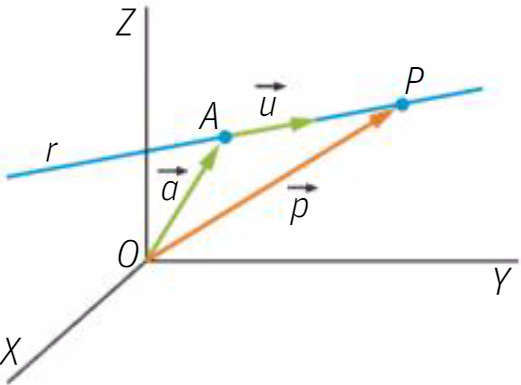
\includegraphics[width=0.4\textwidth]{img/EcVectorialRecta.png}
    \caption{Representación gráfica de la ecuación vectorial de la recta.}
    \label{fig::recta_ecuacion_vectorial}
\end{figure}


¿Es posible construir la recta sin ese parámetro $\lambda$? En realidad,
$$\underbrace{r : \vec{p} = \vec{a} + \lambda \vec{u_r}}_{(0)}\dimplies \underbrace{r:\displaystyle \left\{
\begin{array}{c} 
  x = a_1 + \lambda u_1\\
  y = a_2 + \lambda u_2 \\ 
  z = a_3 + \lambda u_3
\end{array}\right\}}_{(1)} \implies \underbrace{r:\frac{x-a_1}{u_1} = \frac{y-a_2}{u_2} = \frac{z-a_3}{u_3}}_{(2)}$$

\begin{itemize}
    \item A $(1)$ lo denominamos \concept[Ecuación de la recta\IS paramétrica]{ecuación paramétrica de la recta}
    \item A $(2)$ lo denominamos \concept[Ecuación de la recta\IS continua]{ecuación continua de la recta}
\end{itemize}

\[
\frac{x-a_1}{u_1} = \frac{y-a_2}{u_2} = \frac{z-a_3}{u_3}\overset{(1)}{\implies} \left\{
\begin{array}{c}
     \displaystyle\frac{x-a_1}{u_1} = \frac{y-a_2}{u_2}\\
     \displaystyle\frac{y-a_2}{u_2} = \frac{z-a_3}{u_3}
\end{array}\right\} \implies
\underbrace{\left\{\begin{array}{cccc}
     Ax + &By    &     & = D\\
          &B'y   &+ C'z  & = D
\end{array}\right\}}_{(2)}
\]



Donde:
\begin{itemize}
    \item (1) \hide{Se han elegido estas 2 parejas, pero podrían haberse elegido otras, dando lugar a otras ecuaciones implícitas de la misma recta.}
    \item (2) \hide{\concept[Ecuación de la recta\IS implícita]{ecuación implícita de la recta}}
    \subitem \obs \hide{Si interpretáramos las ecuaciones implícitas de la recta como un sistema de ecuaciones, tendríamos un sistema compatible indeterminado con grado de libertad 1.}
    \subitem \obs La dimensión de la recta es 1. \emph{¿Como el grado de indeterminación? Guau...}
\end{itemize}

\begin{problem}
    \ppart 
    Halla todas las ecuaciones de la recta que pasa por $A(0,1,2)$ y es paralela a la que pasa por $B(1,-2,-1)$ y $C(1,0,0)$
    \ppart 
    Halla un vector director de la recta $r:\displaystyle\frac{x-2}{1} = \frac{y-3}{5} = \frac{z-1}{4}$
    \ppart 
    Halla un vector director de la recta $r:\displaystyle\left\{\begin{array}{c} 2x+3y=4\\2x-y+3z=0\end{array}\right\}$
    \solution

\end{problem}

\textbf{Ejercicios:} 
\begin{itemize}
  \item Página 279.13,14.
  \item Página 281.18-21.
\end{itemize}

\subsubsection{Ecuaciones del plano}

Un plano queda determinado por \hide{un punto y dos vectores linealmente independientes}

La 
%
\concept[Ecuación del plano\IS vectorial]{ecuación vectorial del plano} 
%
$\pi$ determinada por el punto $A\in\mathcal{E}_3$ y los vectores linealmente independientes $\vec{V_{\pi}}\in\mathcal{V}^3$ y $\vec{W_{\pi}}\in\mathcal{V}^3$  es $r : \vec{p} = \vec{A} + \lambda \vec{V_{\pi}} + \mu\vec{W_{\pi}}$, con $\lambda\in\real$ (ver ). De esta manera quedan determinados los vectores de posición de todos los puntos del plano.

\begin{figure}[hptb]
    \centering
    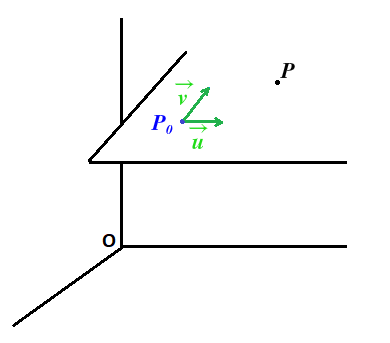
\includegraphics[width=0.65\textwidth]{img/ecplanos.png}
    \caption{Plano generado por un punto y dos vectores}
    \label{fig:plano}
\end{figure}


\paragraph{¿Sería posible evitar el parámetro $\lambda$?} Como en el caso de la recta, podemos escribir esta ecuación en forma de sistema:

$$\pi : \vec{p} = \vec{A} + \lambda \vec{V_{\pi}} + \mu\vec{W_{\pi}}\dimplies \underbrace{\pi:\displaystyle \left\{\begin{array}{c} x = a_1 + \lambda v_1 + \mu w_1\\y = a_2 + \lambda v_2 + \mu w_2 \\ z = a_3 + \lambda v_3 + \mu w_3 \end{array}\right\}}_{(1)} $$

 A $(1)$ lo denominamos \concept[Ecuación del plano\IS paramétrica]{ecuación paramétrica del plano}

\[
\pi:\displaystyle \left\{
\begin{array}{c} 
x - a_1 = \lambda v_1 + \mu w_1\\
y - a_2 = \lambda v_2 + \mu w_2 \\ 
z - a_3 = \lambda v_3 + \mu w_3 
\end{array}\right\}
\]
Como los vectores $\vec{v},\vec{w}$ son linealmente independientes y el vector $AX$ es una combinación lineal de los otros 2 (ver \ref{fig::ecuacion_implicita_plano}), tenemos:


\begin{figure}[hptb]
    \centering
    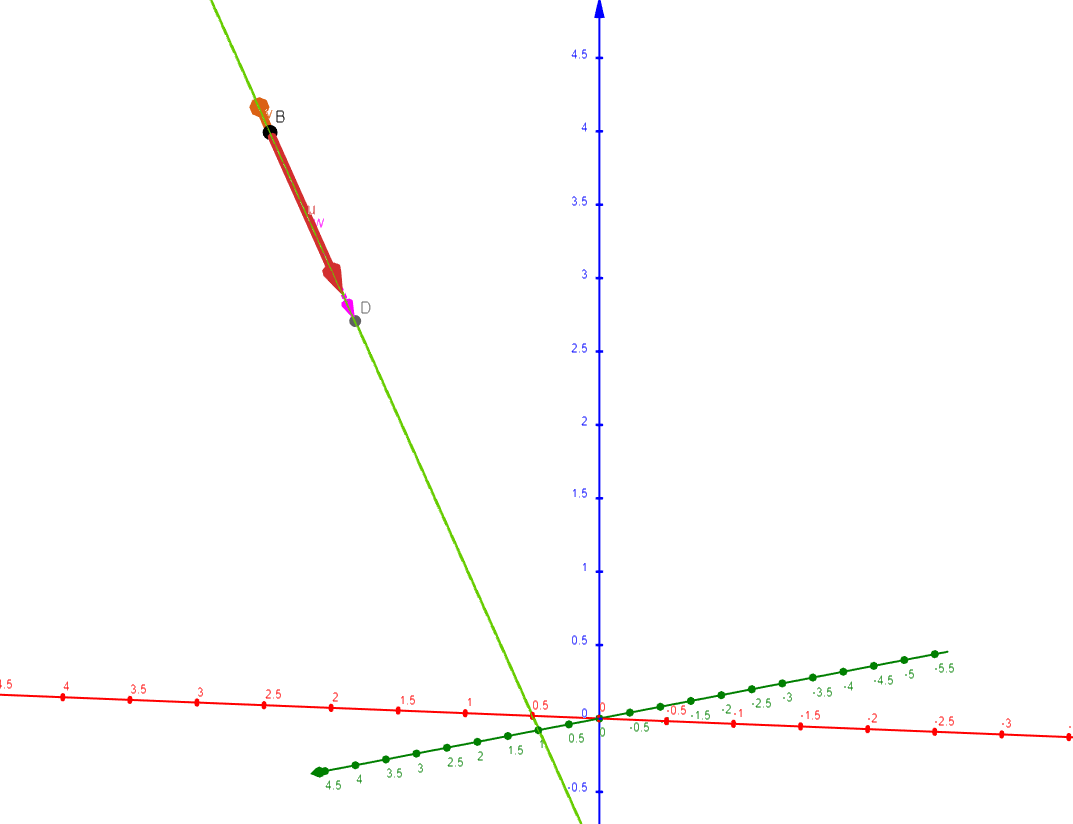
\includegraphics[width=0.3\textwidth]{img/Implicita1.PNG}
    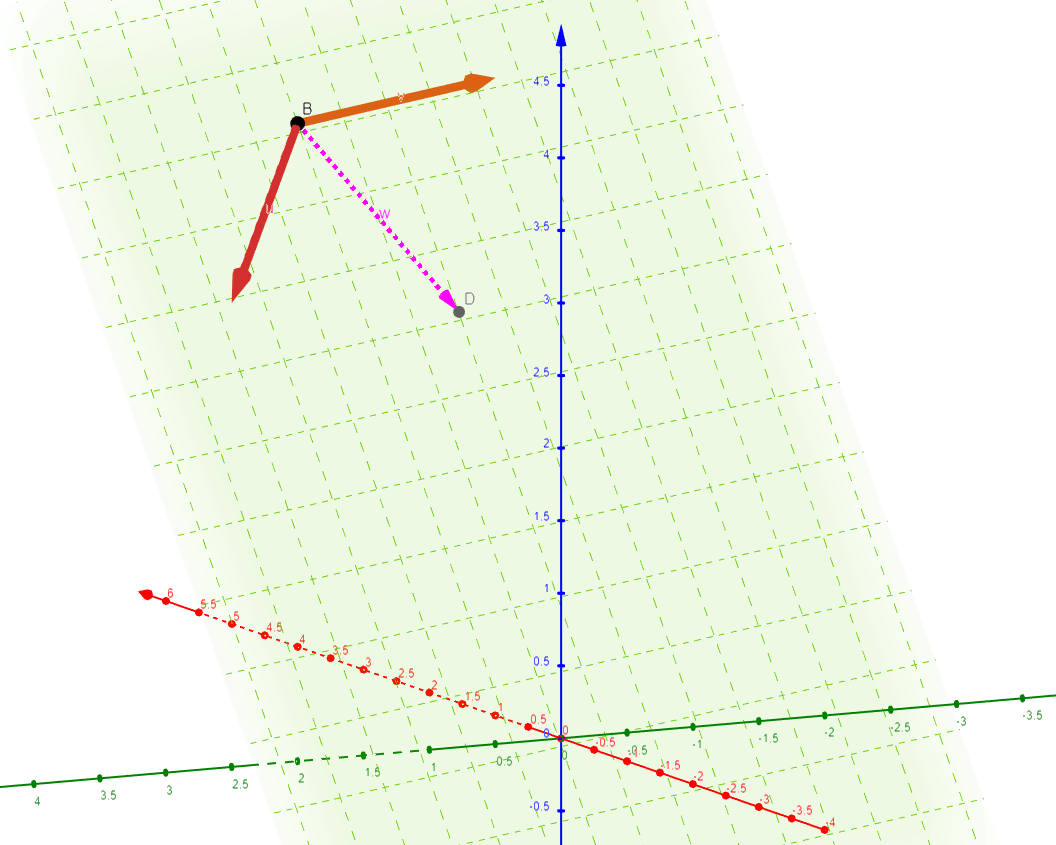
\includegraphics[width=0.4\textwidth]{img/Implicita2.PNG}
    \caption{En la figura de la izquierda puede comprobarse que el vector rosa pertenece al plano, formado por el punto en común y los otros 2 vectores (naranjas). La versión tridimensional se encuentra en \href{https://www.geogebra.org/m/pyh6nnsp}{https://www.geogebra.org/m/pyh6nnsp}.}
    \label{fig::ecuacion_implicita_plano}
\end{figure}

\[
\left|
\begin{array}{ccc} 
x - a_1 & v_1 & w_1\\
y - a_2 & v_2 & w_2 \\ 
z - a_3 & v_3 & w_3 
\end{array}\right| = 0
\]

Desarrollando esta ecuación, tendríamos una ecuación del tipo $Ax+By+Cz + D = 0$, que llamamos \concept[Ecuación del plano\IS implícita]{Ecuación implícita del plano}.



\begin{problem}
    \textbf{Calcula las ecuaciones del plano que pasa por los puntos $A(1,1,1), B(2,2,2), C(1,2,3)$}

    \solution 

    \hide{
    El primer paso sería calcular 2 vectores linealmente independientes de estos 3 puntos, para comprobar que los 3 puntos forman un plano (y no una recta).

    $\vec{AB} = (1,1,1) \quad\quad \vec{AC} = (0,1,2)$, que son linealmente independientes al no ser proporcionales.

    Ecuación vectorial: $\pi: \vec{p} = (1,1,1) + \mu\cdot\vec{AB} + \lambda\cdot\vec{AC}$ con $\lambda,\mu\in\real$

    Ecuación paramétrica: $
    \displaystyle\left\{ \begin{array}{c}
      x = 1 + \mu\\
      y = 1 + \mu + \lambda\\
      z = 1 + \mu + 2\lambda
    \end{array} \right\}\text{ con } \lambda,\mu\in\real$

    Ecuación implícita: 

    \[
      \displaystyle \begin{vmatrix}
      x - 1 & 1 & 0\\
      y - 1 & 1 & 1\\
      z - 1 & 1 & 2\\
    \end{vmatrix} = 0 \dimplies \cdots \dimplies x - 2y+z=0
    \]
    }
\end{problem}


\begin{problem}
\ppart Halla la ecuación de 2 rectas que pertenezcan al mismo plano.
\ppart Halla un vector director del plano: $\pi_1: x+y+z = 3$
\ppart Halla el plano paralelo a $\pi_2: x+y+z = 3$ que pase por el origen de coordenadas.
\ppart Halla el plano paralelo al $XY$ que pasa por $A(-1,2,-2)$.
\obs Llamamos plano $XY$ al plano "del suelo", es decir, al plano $z=0$.

\ppart Página 283, ejercicios 25-28.

\solution

\end{problem}

\subsection{Posiciones relativas}

\subsubsection{Entre 2 planos}  

\begin{framed}
\textbf{Ecuaciones vectoriales o paramétricas:} A continuación, se ofrecen algunos criterios para realizar el estudio de la posición relativa de dos planos.
  \begin{itemize}
    \item Si 2 planos comparten 3 puntos, entonces son el mismo plano.
    \item Si la matriz formada por los 4 vectores directores de los 2 planos tiene rango 2, los planos son paralelos.
    \item Si 2 planos paralelos comparten un punto, entonces son coincidentes.
    \item Si la matriz formada por los 4 vectores directores de los 2 planos tiene rango 3, los planos son secantes en una recta.
    \item \textit{Criterio de perpendicularidad}
  \end{itemize}
\end{framed}



\subparagraph{Ecuaciones implícitas:} En el caso concreto de que los 2 planos estén expresados en ecuaciones implícitas, podremos estudiar su posición relativa discutiendo el sistema formado por ambas ecuaciones:

\[
\left\{\begin{array}{c}
\pi_1: Ax+By+Cz = D\\
\pi_2: A'x+B'y+C'z = D'
\end{array}\right\}
\]

Obtenemos las matrices: $M = \displaystyle\begin{pmatrix}A&B&C\\A'&B'&C'\end{pmatrix}$ y $M^* = \displaystyle\begin{pmatrix}A&B&C&D\\A'&B'&C'&D'\end{pmatrix}$

\begin{framed}
  \begin{itemize}
    \item $Rg(M) = Rg(M^*) = 1 $\hide{ coincidentes.}
    \item $Rg(M) < Rg(M^*) = 2 $\hide{ paralelos.}
    \item $Rg(M) = Rg(M^*) = 2 $\hide{ secantes.}
  \end{itemize}
\obs Las ecuaciones implícitas de la recta, en realidad, es la expresión de 2 planos secantes (que, como no puede ser de otra manera, forman una recta)
\end{framed}

\begin{problem}
Estudia la posición relativa de los siguientes planos:

\[
\pi: \left\{\begin{matrix}x=\lambda+\mu\\y=1-\lambda\\z=2-2\lambda+\mu\end{matrix}\right\}
\]
\[
\pi': x-2y+z=1
\]

\solution

%\vspace{10cm}

\end{problem}

\subsubsection{Entre 3 planos}

\subparagraph{Ecuaciones vectorial o paramétricas}

El estudio de posición relativa en este caso se hace demasiado complejo. Es preferible pasar los planos a ecuaciones implícitas para el estudio.

\subparagraph{Ecuaciones implícitas} Como antes, discutiremos el sistema formado por las ecuaciones implícitas del plano.

\[
\left\{\begin{array}{c}
\pi_1: Ax+By+Cz = D\\
\pi_2: A'x+B'y+C'z = D'\\
\pi_3: A''x+B''y+C''z = D''\\
\end{array}\right\}
\]

Obtenemos las matrices: 
$M  = \displaystyle\begin{pmatrix}
A&B&C\\
A'&B'&C'\\
A''&B''&C''
\end{pmatrix}
$ y 
$M^* = \displaystyle\begin{pmatrix}
A&B&C&D\\
A'&B'&C'&D'\\
A''&B''&C''&D''
\end{pmatrix}
$

Las posibilidades son: (ver figura \ref{fig:PosicionesRelativasPlanos})
\begin{framed}
  \begin{itemize}
    \item $Rg(M) = Rg(M^*) = 1 $\hide{ SCI, secantes en un plano [grado de indeterminación 2, por lo que hay dos parámetros. \textbf{Coincidentes}.}
    \item $Rg(M) < Rg(M^*) = 2 $\hide{ paralelos.}
    \item $Rg(M) = Rg(M^*) = 2 $\hide{ SCI, secantes en una recta [grado de indeterminación 1, por lo que hay un parámetro.}
    \item $Rg(M) = 2 < Rg(M^*) = 3 $\hide{ no se cortan los 3. Sistema incompatible}
    \item $Rg(M) = Rg(M^*) = 3 $\hide{ SCD, secantes en un punto que es la solución del sistema.}
  \end{itemize}  
\end{framed}

\newpage
\begin{figure}[hptb]
    \centering
    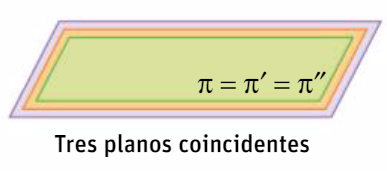
\includegraphics[width=0.65\textwidth]{img/Captura1.png}
    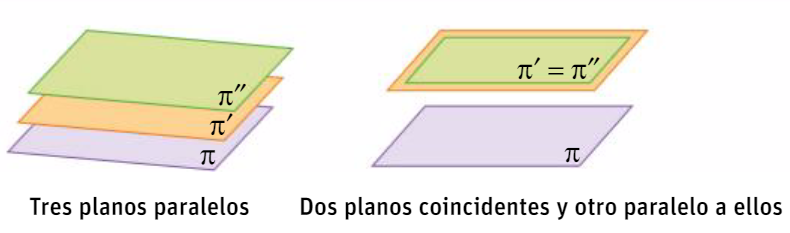
\includegraphics[width=0.95\textwidth]{img/Captura2.png}
    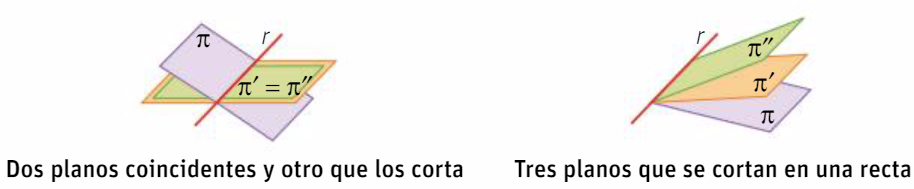
\includegraphics[width=1.1\textwidth]{img/Captura3.png}
    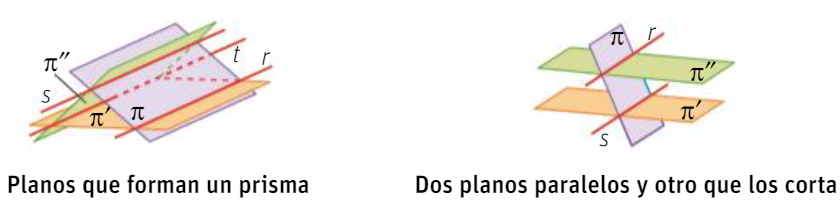
\includegraphics[width=1.1\textwidth]{img/Captura4.png}
    \caption{Representación gráfica de las posiciones relativas de 3 planos.}
    \label{fig:PosicionesRelativasPlanos}
\end{figure}


\begin{problem}
Estudia la posición relativa de los planos: 
\begin{align*}
\pi_1: 2x-3y+2z=7\\
\pi_2: -3+y-z=-5\\
\pi_3:2x-2x+3z=7
\end{align*}
\solution

\begin{align*}
\left\{
\begin{array}{c}
    \pi_1: 2x-3y+2z=7\\
    \pi_2: -3+y-z=-5\\
    \pi_3:2x-2x+3z=7
\end{array}
\right\} \to
\left\|
\begin{array}{c}
M = \begin{pmatrix}             2&-3&2\\-3&1&-1\\2&-2&3
\end{pmatrix} \\\\
M' = \begin{pmatrix}             2&-3&2&-7\\-3&1&-1&5\\2&-2&3&-7
\end{pmatrix} \end{array}\right.
\end{align*}

%\vspace{10cm}

\end{problem}


\subsubsection{Posiciones relativas entre recta y plano}

\paragraph{Ecuaciones implícitas: } Si la recta y como el plano están dados en ecuaciones implícitas, estaríamos en la posición relativa de 3 planos, sabiendo que 2 de ellos son secantes en una recta.

\paragraph{Ecuaciones paramétrica: } $\pi: \{P_{\pi},\vec{v_{\pi}}, \vec{w_{\pi}}\}$ 

\begin{center}
\begin{tabular}{ccc}
$P_r \in \pi $ & $\vec{v_r}$ LD de $v_{\pi}, \vec{w}_{\pi}$ & \textbf{Conclusión}\\\hline
No & No & Secantes en un punto\\
No & Sí & Recta paralela\\
Sí & No & Secantes en un punto\\
Sí & Sí & Recta contenida en el plano\\
\end{tabular}
\end{center}

\begin{problem}
Dada la recta $r: \left\{\begin{array}{c}
    x=\lambda\\
    y=1-2\lambda\\
    z=2
\end{array}\right\}$ y el plano $\pi: (0,1,1) + \mu\cdot (-1,0,0) + \lambda\cdot(2,0,1)$ 
\solution
%\vspace{10cm}

\end{problem}

\paragraph{Plano implícito, recta paramétrica: } comprobamos si existe algún valor de $\lambda_{r}$ para el que se cumpla la ecuación implícita del plano. 
\begin{itemize}
  \item $\exists!\lambda \implies $ secante.
  \item $\lambda \in \real \implies$ contenida.
  \item $\not\exists \lambda \implies $ paralela.
\end{itemize}
\begin{problem}
Estudia la posición relativa del plano $\pi: 2x-2y+z=0$ y de ña recta $r:\left\{\begin{array}{c}
     x=1-2\lambda\\
     y=1+2\lambda\\
     z=3+5\lambda 
\end{array}\right\}$
\solution

%\vspace{10cm}

\end{problem}

\begin{problem}
Estudia la posición relativa del plano $\pi: 2x-2y+z=0$ y de ña recta $r:\left\{\begin{array}{c}
     x=1+\lambda\\
     y=-2+2\lambda\\
     z=3-\lambda 
\end{array}\right\}$
\solution

Sustituimos los valores de $x,y,z$ de las ecuaciones de $r$ en el plano $\pi$:

\[3(1+\lambda) - (-2+2\lambda) + 3 - \lambda = 0 \dimplies 3+3\lambda+2-2\lambda-2\lambda+3-\lambda \dimplies 8=0\]

\textbf{Conclusión} La recta y el plano no tienen nada en común, por lo que tienen que ser paralelos.

\end{problem}


Ejercicios recomendados: 105ab,107ab

\subsubsection{Posiciones relativas entre dos rectas}

Las distintas posibilidades de posición relativa son:

  \begin{tabular}{c|c|c}
\textbf{Posición relativa} & \textbf{Vectores} &\textbf{ Puntos}\\\hline
Paralelas coincidentes & Paralelos & Todos en común (*)\\
Paralelas no coincidentes. & Paralelos & Ninguno en común\\
Secantes en un punto & No paralelos & Solamente uno en común.\\
Se cruzan en el espacio & No paralelos & Ninguno en común\\
\end{tabular}

\begin{figure}[hptb]
    \centering
    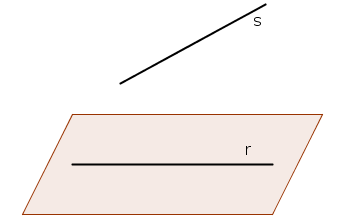
\includegraphics[width=0.4\textwidth]{img/rectasquesecruzan.png}
    \caption{Representación gráfica de dos rectas que se cruzan en el espacio.}
    \label{fig::rectas_que_se_cruzan_en_el_espacio}
\end{figure}


\begin{framed}
  Dadas las rectas 
$r:\vec{p} = \vec{a} + \lambda\vec{u},\quad \lambda\in\real$
y
$s:\vec{p} = \vec{b} + \lambda\vec{w},\quad \lambda\in\real$. 


\begin{itemize}
    \item $\vec{u}|| \vec{w} \to $ Paralelas o coincidentes.
    \subitem $A_r\in s$ ó $B_s\in r \implies$ coincidentes.
    \subitem En caso contrario, paralelas no coincidentes.
    \item $\vec{u}\not || \vec{w} \to $ secantes o se cruzan.
    \subitem Ver \textit{procedimiento general}.
\end{itemize}
\end{framed}

\paragraph{Procedimiento general:}
\label{txt::procedimiento_general}

Si los vectores directores son paralelos (proporcionales), las rectas pueden ser paralelas o coincidentes. 
%
Para poder distinguir, podríamos ver si un vector formado por un punto de cada recta es también proporcional (entonces serían coincidentes) o si no (entonces serían secantes).

De la misma manera, si los vectores son linealmente independientes las rectas pueden cruzarse o cortarse. 
%
Para distinguir estos 2 casos, podríamos ver si un vector formado por un punto de cada recta es linealmente dependiente a los otros 2 (entonces serían secantes porque formarían un plano que contiene al vector) o si no (entonces se cortarían en el espacio).

Así, buscamos estudiar la dependencia lineal de los 2 vectores directores ($\vec{u},\vec{w}$) y de los 2 vectores directores respecto de un vector formado, arbitrariamente, con 2 puntos de las rectas ($\vec{AB}$, con $A(a_1,a_2,a_3)\in r$ y $B(b_1,b_2,b_3)\in s$). 
%
Para ello, formamos las matrices:

$M  = \displaystyle\begin{pmatrix}
u_1&w_1\\
u_2&w_2\\
u_3&w_3
\end{pmatrix}
$ y 
$M^* = \displaystyle\begin{pmatrix}
u_1&w_1&b_1-a_1\\
u_2&w_2&b_2-a_2\\
u_3&w_3&b_3-a_3\\
\end{pmatrix}
$

\begin{framed}
  \begin{itemize}
    \item $Rg(M) = Rg(M^*) = 1 $\hide{ SCI, secantes en una recta [grado de indeterminación 1, por lo que hay dos parámetros.] \textbf{Coincidentes}.]}
    \item $Rg(M) = 1 < Rg(M^*) = 2 $\hide{ paralelas.} 
    \item $Rg(M) = Rg(M^*) = 2 $\hide{ SCI, secantes en un plano [dimensión 2]. $\vec{AB}$ se puede escribir como combinación lineal de $\vec{u}$ y $\vec{w}$}
    \item $Rg(M) = 2 < Rg(M^*) = 3 $\hide{ se cruzan en el espacio.} 
  \end{itemize}  
\end{framed}

\begin{problem}
Estudia la posición relativa de las siguientes rectas:

\[
r:\left\{
\begin{array}{c}
x=\lambda \\
y=-1+2\lambda\\
z=1-\lambda
\end{array}
\right\}
\;\;\;\;
s:\left\{
\begin{array}{c}
x=2\lambda \\
y=2+\lambda\\
z=2-3\lambda
\end{array}
\right\}
\]
\solution

Se toma un punto y un vector de cada recta:
\[
r: A(0,-1,1), \vec{u_r} =(1,2,-1)\quad\quad s: B(0,2,2), \vec{w_s} = (2,1,-3)
\]

Se consideran las matrices: $M=\left(\vec{u_r}, \vec{w_s}\right) \quad M^\ast = \left(\vec{u_r},\vec{w_s}, [\vec{AB}]\right)$ y se estudia el rango.

%\vspace{5cm}

Para hallar las coordenadas el punto de corte: 

%\vspace{5cm}

\end{problem}

\begin{problem}
Página 289, ejercicios 52, calculando puntos de cortes
\solution
\end{problem}


\paragraph{Ambas rectas en general:} 
%
Formamos la matriz de 4x4 y estudiamos la posición relativa de 4 planos.
%
Consultando \fref{fig:PosicionesRelativasPlanos} tenemos todos los casos cubiertos en los que uno de los planos es combinación lineal de los demás. 
%
En el caso en el que no haya ningún plano que sea combinación lineal de los demás, tendremos que la matriz ampliada tendrá rango 4 por lo que el sistema será incompatible. 
%
Geométricamente, tendremos rectas que se cruzan.

\begin{problem}
Estudia la posición relativa de las siguientes rectas:
\[
r: 
\left\{
\begin{array}{l}
x+y+z=1\\
-3x+y+z=1
\end{array}
\right\}\;\;\;\;
s: 
\left\{
\begin{array}{l}
2x-y+z=1\\
-x+z=0
\end{array}
\right\}
\]
\solution

\[
\left\{
\begin{array}{l}
x+y+z=1\\
-3x+y+z=1\\
2x-y+z=1\\
-x+z=0
\end{array}
\right\} \to M^\ast=\begin{pmatrix}
0&1&1&1\\-3&1&1&1\\2&-1&1&1\\-1&0&1&0
\end{pmatrix}
\]

Calculamos $|M^\ast|$
\[
|M^\ast|=\begin{pmatrix}
0&1&1&1\\-3&1&1&1\\2&-1&1&1\\-1&0&1&0
\end{pmatrix} = ... = -6
\]

$Rg(M) \leq 3 < 4 = Rg(M^\ast)$, por lo que el sistema es incompatible.
%
Por ello, las rectas se cruzan en el espacio.

\end{problem}

\paragraph{Haz de rectas}
%\paragraph{Haz de rectas paralelas: } cambia el punto, manteniendo fijo el vector. 
%\paragraph{Haz de rectas secantes: } cambia el vector (sin ser nunca nulo), mantiene fijo el punto.
%\paragraph{Haz de planos paralelelos: } cambia el punto, mantiene los vectores
%\paragraph{Haz de planos secantes en una recta: } mantiene un vector y un punto, cambia el otro vector.

%\begin{problem}
%Tema 11: 56,57,59,60.
%\solution
%\end{problem}

%Deberes: 118,136,143


\paragraph{Practicamos en general}
Tema 11: 
122,127,130,134,135,136,139,140,143,145,149,150

Tema 11:
\begin{itemize}
  \item Básicos: 83,91,92,93a,98,100,101a,103a,104a,105,106,107d,108
  \item Síntesis: 111-119
  \item Completos: 122-124,127,129-133
\end{itemize}



